% Options for packages loaded elsewhere
\PassOptionsToPackage{unicode}{hyperref}
\PassOptionsToPackage{hyphens}{url}
%
\documentclass[
  12pt,
]{article}
\usepackage{lmodern}
\usepackage{amssymb,amsmath}
\usepackage{ifxetex,ifluatex}
\ifnum 0\ifxetex 1\fi\ifluatex 1\fi=0 % if pdftex
  \usepackage[T1]{fontenc}
  \usepackage[utf8]{inputenc}
  \usepackage{textcomp} % provide euro and other symbols
\else % if luatex or xetex
  \usepackage{unicode-math}
  \defaultfontfeatures{Scale=MatchLowercase}
  \defaultfontfeatures[\rmfamily]{Ligatures=TeX,Scale=1}
  \setmainfont[]{Times New Roman}
\fi
% Use upquote if available, for straight quotes in verbatim environments
\IfFileExists{upquote.sty}{\usepackage{upquote}}{}
\IfFileExists{microtype.sty}{% use microtype if available
  \usepackage[]{microtype}
  \UseMicrotypeSet[protrusion]{basicmath} % disable protrusion for tt fonts
}{}
\makeatletter
\@ifundefined{KOMAClassName}{% if non-KOMA class
  \IfFileExists{parskip.sty}{%
    \usepackage{parskip}
  }{% else
    \setlength{\parindent}{0pt}
    \setlength{\parskip}{6pt plus 2pt minus 1pt}}
}{% if KOMA class
  \KOMAoptions{parskip=half}}
\makeatother
\usepackage{xcolor}
\IfFileExists{xurl.sty}{\usepackage{xurl}}{} % add URL line breaks if available
\IfFileExists{bookmark.sty}{\usepackage{bookmark}}{\usepackage{hyperref}}
\hypersetup{
  pdftitle={Comparison of Effects of COVID-19 on Counties With and Without Coal Mines},
  pdfauthor={Thomas Hancock},
  hidelinks,
  pdfcreator={LaTeX via pandoc}}
\urlstyle{same} % disable monospaced font for URLs
\usepackage[margin=2.54cm]{geometry}
\usepackage{longtable,booktabs}
% Correct order of tables after \paragraph or \subparagraph
\usepackage{etoolbox}
\makeatletter
\patchcmd\longtable{\par}{\if@noskipsec\mbox{}\fi\par}{}{}
\makeatother
% Allow footnotes in longtable head/foot
\IfFileExists{footnotehyper.sty}{\usepackage{footnotehyper}}{\usepackage{footnote}}
\makesavenoteenv{longtable}
\usepackage{graphicx,grffile}
\makeatletter
\def\maxwidth{\ifdim\Gin@nat@width>\linewidth\linewidth\else\Gin@nat@width\fi}
\def\maxheight{\ifdim\Gin@nat@height>\textheight\textheight\else\Gin@nat@height\fi}
\makeatother
% Scale images if necessary, so that they will not overflow the page
% margins by default, and it is still possible to overwrite the defaults
% using explicit options in \includegraphics[width, height, ...]{}
\setkeys{Gin}{width=\maxwidth,height=\maxheight,keepaspectratio}
% Set default figure placement to htbp
\makeatletter
\def\fps@figure{htbp}
\makeatother
\setlength{\emergencystretch}{3em} % prevent overfull lines
\providecommand{\tightlist}{%
  \setlength{\itemsep}{0pt}\setlength{\parskip}{0pt}}
\setcounter{secnumdepth}{5}

\title{Comparison of Effects of COVID-19 on Counties With and Without Coal
Mines}
\usepackage{etoolbox}
\makeatletter
\providecommand{\subtitle}[1]{% add subtitle to \maketitle
  \apptocmd{\@title}{\par {\large #1 \par}}{}{}
}
\makeatother
\subtitle{\url{https://github.com/tnh2/ENV872_Project}}
\author{Thomas Hancock}
\date{}

\begin{document}
\maketitle

\newpage
\tableofcontents 
\newpage
\listoftables 
\newpage
\listoffigures 
\newpage

\hypertarget{rationale-and-research-questions}{%
\section{Rationale and Research
Questions}\label{rationale-and-research-questions}}

The purpose of this analysis is to explore whether counties with coal
mines are impacted differently by COVID-19. With the novel coronavirus
rapidly spreading through the United States, different locations are
likely to be affected in different ways. In order to perform the
analysis, I combined datasets containing information about coal mine
locations, populations, and COVID-19 cases and deaths at the county
level. Because other factors such as socioeconomic levels, population
densities, and even government responses to the COVID-19 crisis vary
widely across states, I decided that it was best to compare counties
within states rather than performing analysis on the entire country. In
particular, I focused on Pennsylvania and West Virginia. Pennsylvania
has had a relatively large number of confirmed COVID-19 cases, meaning
there is a reasonable amount of data to analyze. West Virginia has had
relatively few confirmed cases, but I included it as a comparison to
Pennsylvania since West Virginia coal mines have continued operation
whereas Pennsylvania mines were closed in March \textsuperscript{1}.

I am curious to see if there is any difference in COVID-19 outcomes
between counties with coal mines and those without. In particular, I am
interested in whether or not there will be a difference in mortality
(the percentage of people who have the disease that die from it). The
rational behind this exploration is that COVID-19 seems to be
particularly lethal among people with existing conditions, especially
respiratory issues. In turn, coal miners frequently suffer respiratory
issues from the large amonts of dust that they encounter in their jobs.
As such, I wondered if there might be a higher mortality rate in coal
mining counties than non-coal mining counties (as a proxy for mortality
amongst coal miners versus others). Likewise, coal mining involves
sustained close-quarters operation and minimal opportunity for
sanitization, hence my wanting to compare counties in Pennsylvania where
the mines shut down in response to the outbreak to counties in West
Virginia where mines continued operation.

My research questions are:

\begin{enumerate}
\def\labelenumi{\arabic{enumi}.}
\item
  Do counties with coal mines have different mortality rates than
  similar counties without coal mines in the same state?
\item
  Do counties with coal mines in Pennsylvania have different mortality
  rates than West Virgnia counties with coal mines?
\end{enumerate}

\newpage

\hypertarget{dataset-information}{%
\section{Dataset Information}\label{dataset-information}}

To perform my analysis, I gathered together five datasets: US Census
state and county boundaries (as shapefiles), US Census population data
for US counties, coal mine locations from the US Department of Energy
(as a shapefile), and county-level COVID-19 case and death counts from
the Johns Hopkins University Center for Systems Science and Engineering
(CSSE). The population data from the US Census Bureau are from 2019
estimates. The coal mine information inlcudes all operating surface and
underground mines in the united states. While the dataset includes
information on the mine type and output, I only used the location data
for this analysis. The COVID-19 data from Johns Hopkins includes
confirmed COVID-19 cases and reported deaths by county as of April 23rd,
2020.

I started wrangling my data by finding which counties had coal mines in
them using the geospatial analysis capabilities of the sf package in R.
I then joined the COVID-19 data with the census population data using
the county FIPS codes and calculated metrics for COVID-19 case rates
(per 100,000 people), mortality rate (deaths per confirmed COVID-19
case), and death rates per 100,000 people in the county. This data was
then combined with the data above identifying whether a county had coal
mines or not to complete the data joining. From this country-wide
dataset, I filtered out the data specific to the two states I focused on
for this study (Pennsylvania and West Virginia). The important data
included in these data sets are outlined in Table 1 below.

\begin{longtable}[]{@{}lll@{}}
\caption{Important Data Fields}\tabularnewline
\toprule
Field Name & Description & Units\tabularnewline
\midrule
\endfirsthead
\toprule
Field Name & Description & Units\tabularnewline
\midrule
\endhead
STNAME & State Name &\tabularnewline
CTYNAME & County Name &\tabularnewline
POPESTIMATE2019 & 2019 Estimated Population & People\tabularnewline
FIPS & 5-digit county identifier &\tabularnewline
Confirmed & Confirmed COVID-19 cases & Total Cases\tabularnewline
Deaths & Reported COVID-19 deaths & Total Deaths\tabularnewline
case\_rate & Rate of COVID-19 cases & Cases per 100,000
people\tabularnewline
death\_rate\_conf & Mortality & Deaths per confirmed case\tabularnewline
death\_rate\_pop & Deaths rate in population & Deaths per 100,000
people\tabularnewline
Mines.Label & Whether the County has mines & Mines or No
Mines\tabularnewline
\bottomrule
\end{longtable}

\newpage

\hypertarget{exploratory-analysis}{%
\section{Exploratory Analysis}\label{exploratory-analysis}}

\hypertarget{locational-verification}{%
\subsection{Locational Verification}\label{locational-verification}}

The first step of my analysis was to make sure that the counties with
coal mines were properly identified. To do this verification, I made a
map showing the counties that were identified as having a coal mine on
one layer, and the point locations of the mines on another layer. If the
counties were correctly identified, each of the mine points should be
within one of the coal county boundaries. This map is shown in Figure 1.
As the figure shows, the counties were correctly identified (i.e., no
mines are in a non-coal county and all coal counties have at least one
mine).

\hypertarget{pennsylvania-data}{%
\subsection{Pennsylvania Data}\label{pennsylvania-data}}

Turning my attention to Pennsylvania, I started by creating a histogram
of the mortality rates of the coal counties and the non-coal counties.
The first histogram I created is shown in Figure 1 below.

\begin{figure}
\centering
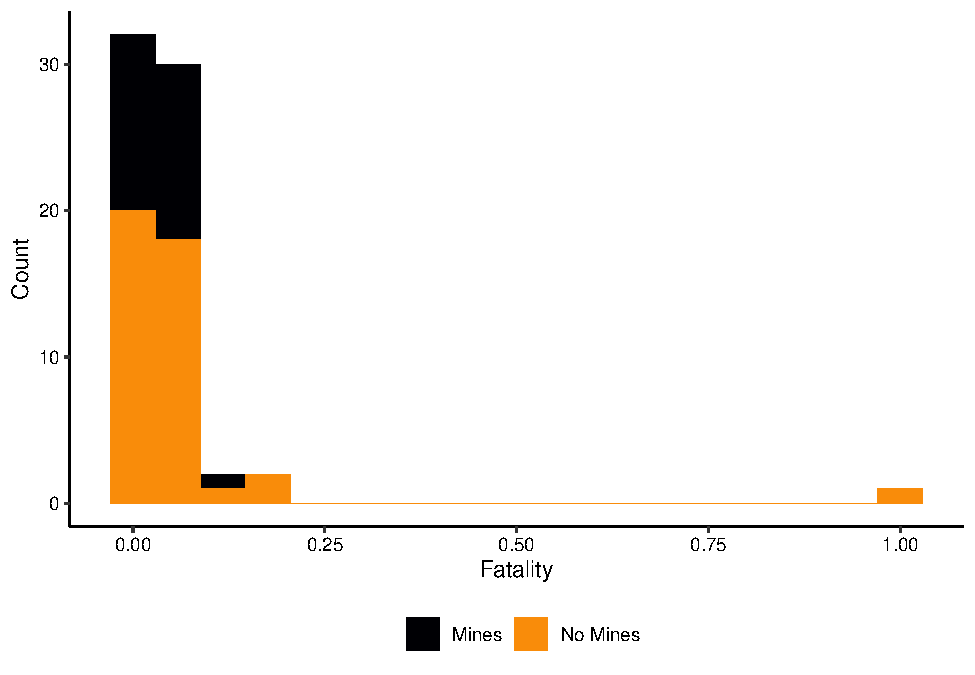
\includegraphics{Hancock_ENV872_Project_files/figure-latex/PA Histogram1-1.pdf}
\caption{Histogram of Mortality in Pennsylvania counties}
\end{figure}

Two things are immediately evident: the data are not normally
distributed, and there are some strange cases where the mortality is 1
(i.e., everyone confirmed case of COVID-19 resulted in a death). Based
on general knowledge that COVID-19 is not likely to be lethal enough to
kill even a majority of patients, we can assume that these counties had
such limited testing that only the mortalities were tested. For the sake
of this analysis, we will discard those counties and any others that
have a mortality rate greater than 50\%. We will assume that the
remaining counties had testing that was sufficiently widespread to
provide a reasonable approximation of the mortality. This new dataset
yields the histogram in Figure 2. The distribution is still not normal,
but it has a smoother shape for both the counties with mines and those
without. There are still a few counties with suspiciously higher
mortality rates, but without further data, there is not enough reason to
remove them.

\begin{figure}
\centering
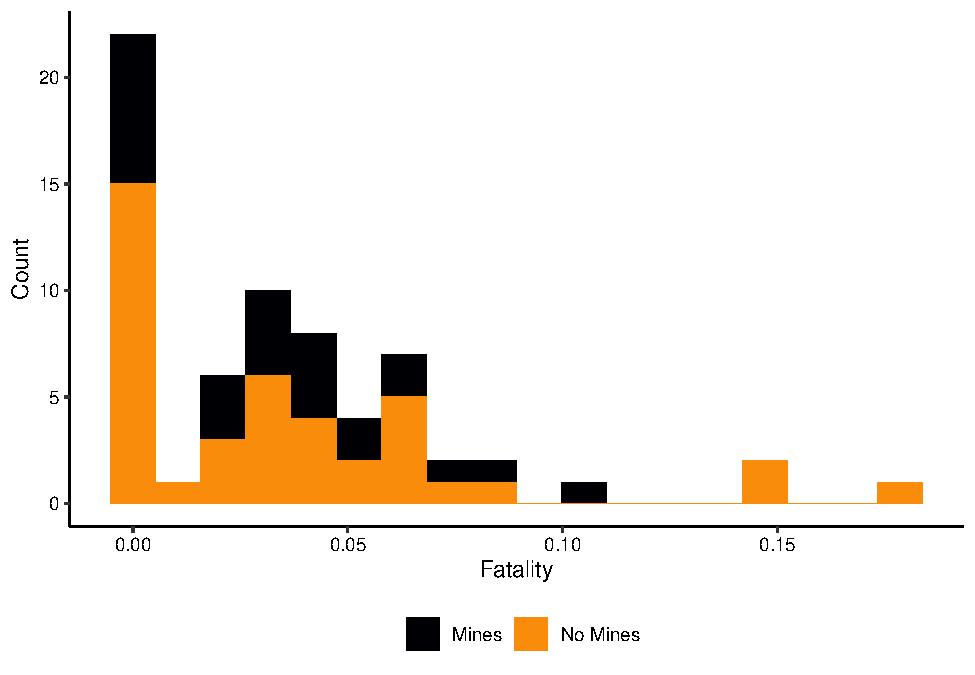
\includegraphics{Hancock_ENV872_Project_files/figure-latex/PA Histogram2-1.pdf}
\caption{Histogram of Mortality in Pennsylvania counties (outliers
removed)}
\end{figure}

I decided to explore the potential relationship between mortality and
the amount of testing by plotting mortality against the number of
confirmed cases per 100,000 people in each county. The results are
presented in Figure 3. Even without the aforementioned counties that
only tested fata cases, there appears to be a slight decreasing trend in
mortality as the confirmed case rate increases. However, this trend is
not statistically significant (linear regression; p-value = 0.395;
F-statistic = 0.7344; degrees of freedom: 1 and 64).

\begin{figure}
\centering
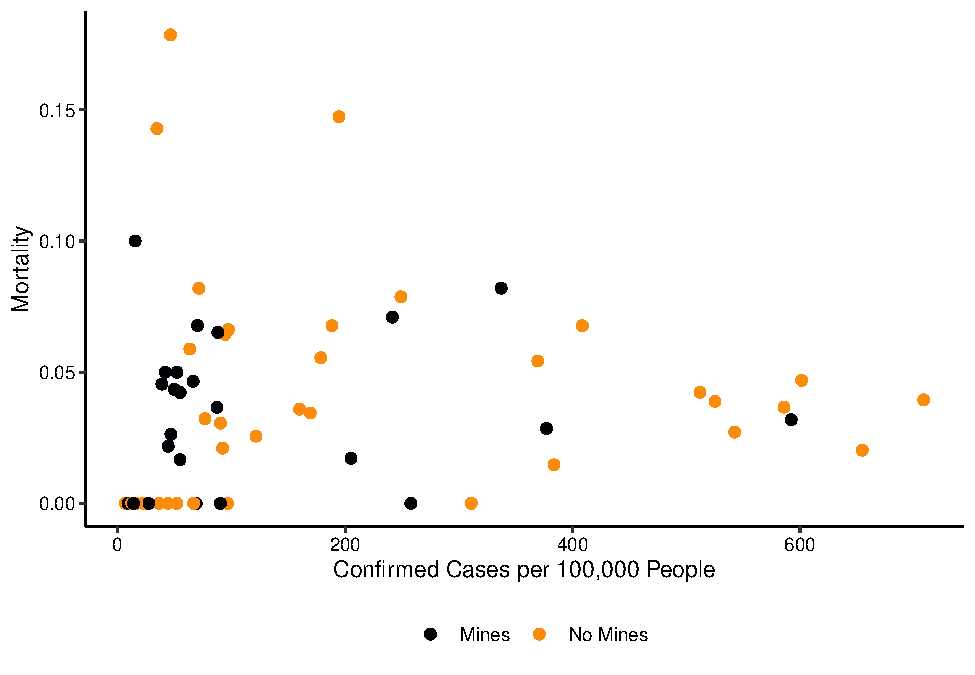
\includegraphics{Hancock_ENV872_Project_files/figure-latex/PA Mortality vs Case Rate-1.pdf}
\caption{Mortality vs confirmed COVID-19 case rate for Pennsylvanian
counties with and without coal mines.}
\end{figure}

\begin{itemize}
\tightlist
\item
  Map
\item
  Histograms
\item
  Scatterplot
\end{itemize}

\hypertarget{west-virginia-data}{%
\subsection{West Virginia Data}\label{west-virginia-data}}

As mentioned earlier, I am also interested in seeing if there is a
difference between West Virginia, where coal mines stayed open despite
the pandemice, and Pennsylvania, where mines were closed. In Figure 5, I
plotted histograms for the West Virginia data, similar to what was done
for Pennsylvania. From these histograms, we can see that there were a
few West Virignia counties that tested mostly fatal cases of COVID-19,
so it is reasonable to perform the same removal of ouliers with
mortality rates above 50\%. Likewise, the West Virginia data has a very
non-normal distribution.

\begin{figure}
\centering
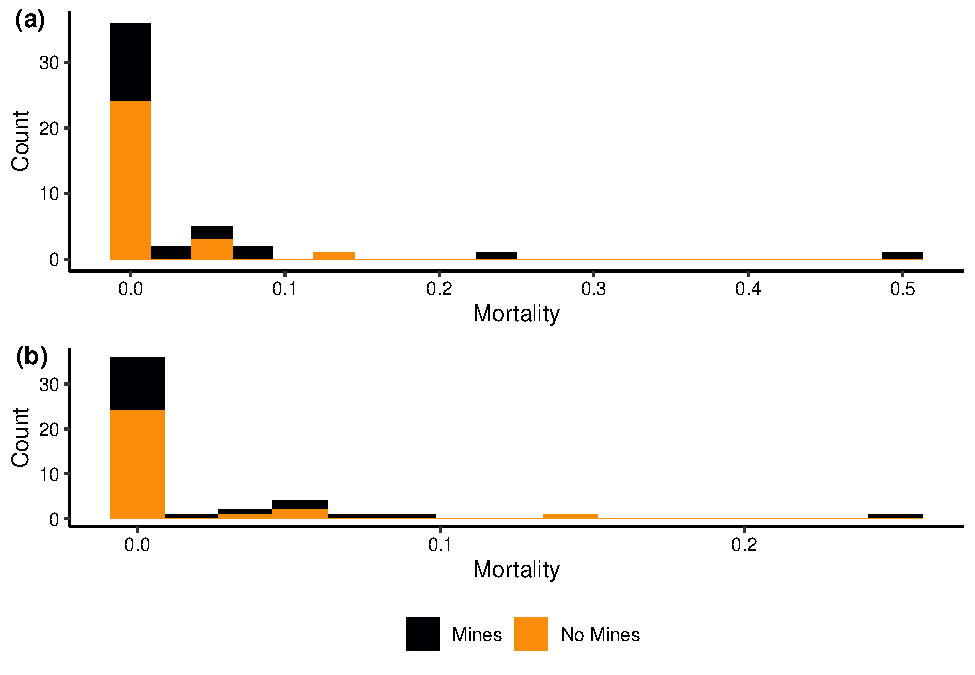
\includegraphics{Hancock_ENV872_Project_files/figure-latex/WV Histograms-1.pdf}
\caption{Histogram of Mortality in West Virginia Counties (a) with
outliers and (b) without outliers.}
\end{figure}

Plotting the mortality against the confirmed case rate for West Virginia
counties, as shown in Figure 6, reveals little structure to the data.
Perhaps the most useful conclusion that can come from this exploration
of the data is that West Virginia has a rather low reported case rate.

\begin{figure}
\centering
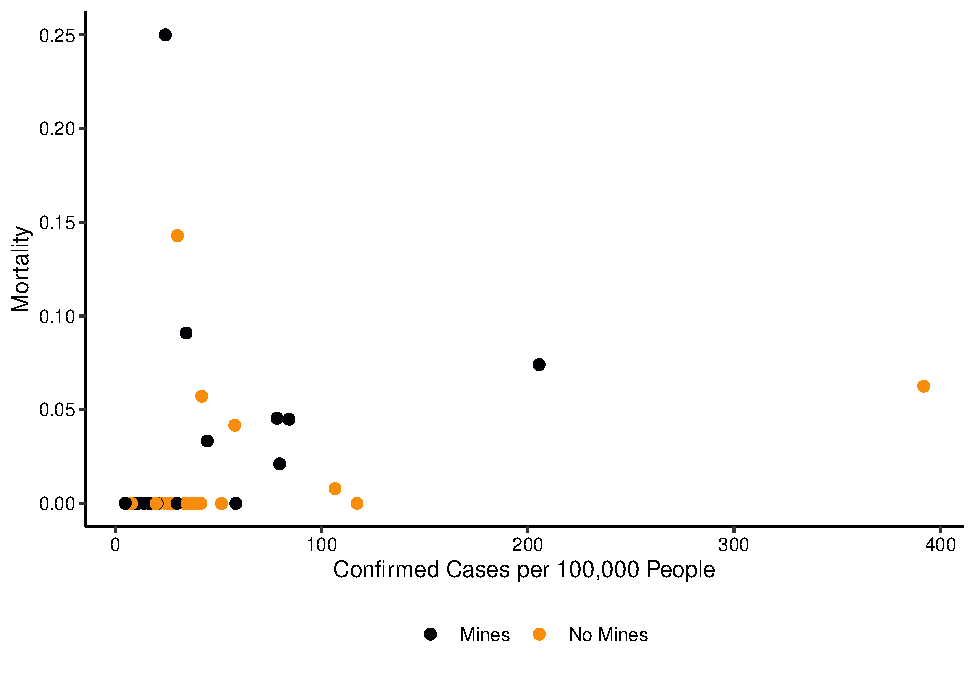
\includegraphics{Hancock_ENV872_Project_files/figure-latex/WV Mortality vs Case Rate-1.pdf}
\caption{Mortality vs confirmed COVID-19 case rate for West Virginian
counties with and without coal mines.}
\end{figure}

\newpage

\hypertarget{analysis}{%
\section{Analysis}\label{analysis}}

\begin{itemize}
\tightlist
\item
  Boxplots
\item
  Wilcoxon results
\end{itemize}

\hypertarget{question-1-do-counties-with-coal-mines-have-different-mortality-rates-than-similar-counties-without-coal-mines-in-the-same-state}{%
\subsection{Question 1: Do counties with coal mines have different
mortality rates than similar counties without coal mines in the same
state?}\label{question-1-do-counties-with-coal-mines-have-different-mortality-rates-than-similar-counties-without-coal-mines-in-the-same-state}}

To answer the first question comparing coal mining counties in
Pennsylvania to non-mining counties, I performed a non-parametric
Wilcoxon test. I chose to use a non-parametric test because the data are
not distributed in a normal distribution (as seen in the Exploration
section). The Wilcoxon uses a ranking system to see if two data sets
have similar shapes.

\hypertarget{question-2-do-counties-with-coal-mines-in-pennsylvania-have-different-mortality-rates-than-west-virgnia-counties-with-coal-mines}{%
\subsection{Question 2: Do counties with coal mines in Pennsylvania have
different mortality rates than West Virgnia counties with coal
mines?}\label{question-2-do-counties-with-coal-mines-in-pennsylvania-have-different-mortality-rates-than-west-virgnia-counties-with-coal-mines}}

\newpage

\hypertarget{summary-and-conclusions}{%
\section{Summary and Conclusions}\label{summary-and-conclusions}}

\begin{itemize}
\tightlist
\item
  No significant differences
\item
  Reasons why this analysis isn't great
\end{itemize}

\newpage

\hypertarget{references}{%
\section{References}\label{references}}

\textless add references here if relevant, otherwise delete this
section\textgreater{}

\end{document}
